\documentclass[a4paper,11pt]{article}
\usepackage{amsmath,amsthm,amsfonts,amssymb,amscd,amstext,vmargin,graphics,graphicx,tabularx,multicol} 
\usepackage[francais]{babel}
\usepackage[utf8]{inputenc}  
\usepackage[T1]{fontenc} 
\usepackage{pstricks-add,tikz,tkz-tab,variations}
\usepackage[autolanguage,np]{numprint} 
\usepackage{calc}

\setmarginsrb{1.5cm}{0.5cm}{1cm}{0.5cm}{0cm}{0cm}{0cm}{0cm} %Gauche, haut, droite, haut
\newcounter{numexo}
\newcommand{\exo}[1]{\stepcounter{numexo}\noindent{\bf Exercice~\thenumexo} : }
\reversemarginpar

\newcommand{\bmul}[1]{\begin{multicols}{#1}}
\newcommand{\emul}{\end{multicols}}

\newcounter{enumtabi}
\newcounter{enumtaba}
\newcommand{\q}{\stepcounter{enumtabi} \theenumtabi.  }
\newcommand{\qa}{\stepcounter{enumtaba} (\alph{enumtaba}) }
\newcommand{\initq}{\setcounter{enumtabi}{0}}
\newcommand{\initqa}{\setcounter{enumtaba}{0}}

\newcommand{\be}{\begin{enumerate}}
\newcommand{\ee}{\end{enumerate}}
\newcommand{\bi}{\begin{itemize}}
\newcommand{\ei}{\end{itemize}}
\newcommand{\bp}{\begin{pspicture*}}
\newcommand{\ep}{\end{pspicture*}}
\newcommand{\bt}{\begin{tabular}}
\newcommand{\et}{\end{tabular}}
\renewcommand{\tabularxcolumn}[1]{>{\centering}m{#1}} %(colonne m{} centrée, au lieu de p par défault) 
\newcommand{\tnl}{\tabularnewline}

\newcommand{\trait}{\noindent \rule{\linewidth}{0.2mm}}
\newcommand{\hs}[1]{\hspace{#1}}
\newcommand{\vs}[1]{\vspace{#1}}

\newcommand{\N}{\mathbb{N}}
\newcommand{\Z}{\mathbb{Z}}
\newcommand{\R}{\mathbb{R}}
\newcommand{\C}{\mathbb{C}}
\newcommand{\Dcal}{\mathcal{D}}
\newcommand{\Ccal}{\mathcal{C}}
\newcommand{\mc}{\mathcal}

\newcommand{\vect}[1]{\overrightarrow{#1}}
\newcommand{\ds}{\displaystyle}
\newcommand{\eq}{\quad \Leftrightarrow \quad}
\newcommand{\vecti}{\vec{\imath}}
\newcommand{\vectj}{\vec{\jmath}}
\newcommand{\Oij}{(O;\vec{\imath}, \vec{\jmath})}
\newcommand{\OIJ}{(O;I,J)}


\newcommand{\reponse}[1][1]{%
\multido{}{#1}{\makebox[\linewidth]{\rule[0pt]{0pt}{20pt}\dotfill}
}}

\newcommand{\titre}[5] 
% #1: titre #2: haut gauche #3: bas gauche #4: haut droite #5: bas droite
{
\noindent #2 \hfill #4 \\
#3 \hfill #5

\vspace{-1.6cm}

\begin{center}\rule{6cm}{0.5mm}\end{center}
\vspace{0.2cm}
\begin{center}{\large{\textbf{#1}}}\end{center}
\begin{center}\rule{6cm}{0.5mm}\end{center}
}



\begin{document}
\pagestyle{empty}
\titre{Séance d'AP 1 : Priorités opératoires}{}{}{4ème}{}

\vspace*{0.2cm}

\setlength{\fboxrule}{2pt}
\begin{flushleft}
\framebox{\begin{minipage}{\linewidth}

\vspace*{0.2cm}

\underline{\textbf{Rappels de cours}}\\

\bi


\item Dans un calcul avec des parenthèses, on effectue en priorité les calculs à l'intérieur des parenthèses.\\

\item Dans un calcul parenthèses, les multiplications et les divisions sont prioritaires sur les additions et les soustractions.\\




\ei

\vspace*{0.2cm}
\end{minipage}}
\end{flushleft}

\vspace*{0.7cm}

\exo  \\
Calculer les expressions suivantes \textbf{en détaillant vos étapes de calculs}.

\bmul{3}

$R = 21 - ( 13 - (4\times 2))$ \\
\reponse[3]\\

\columnbreak

$U = 37 + 21 \div 7$ \\
\reponse[3]\\

\columnbreak

$I = 100 - 48 \div 4\times3$ \\
\reponse[3]\\

\emul

\bmul{2}

$A = \dfrac{104-29}{20-6 \times 3}$ \\
\reponse[3]\\



\columnbreak

$M = (14,2 \times 100 + 0,025 \times 1 000) \times 2$ \\
\reponse[3]\\



\emul



\vspace*{0.5cm}


\exo\\
Compléter la grille ci-dessous.

\bmul{2}

\includegraphics[scale=0.7]{motcroise1.eps} 

\columnbreak



\textbf{Verticalement}\\

\textbf{1.}  $21,3 \times 31 - 17,3 + 1 929$\\

\textbf{4.} $\dfrac{\dfrac{210}{7}}{5} \times (1 000 - 9)$\\

\vspace*{0.2cm}

\textbf{Horizontalement}\\

\textbf{a.}  $5 \times (5 + 36 \times 11)$\\

\textbf{c.} $(14 521 - 13 202) \times (48 \div 12 \times 3 - 6)$\\

\textbf{d.} $11 \times (11 - 4) \times (11 + 2) \times (11 - 9) + 4 $ \\

 \emul

\newpage

\exo\\
 Charlotte   a   effectué   un   calcul   sur   son cahier   sans   se  tromper.   Hélas,   son   père   a renversé   son   café   et   a   fait   de   nombreuses éclaboussures sur son cahier.
 
 \bmul{2}
 
\vspace*{0.2cm}


\includegraphics[scale=0.73]{tachecafe.eps}  

\columnbreak


Réécrire le calcul de Charlotte dans son intégralité.\\
\reponse[6]

\emul




\vspace*{1.2cm}

\underline{\textbf{{\large A faire pour le mercredi 19 septembre :}}}\\

\vspace*{0.4cm}


\exo \\ Calculer les expressions suivantes en respectant les priorités opératoires.\\

\bmul{2}

$T = 4 \times (2 + 3 \times 6) \times 5$ \\
\reponse[6]\\



\columnbreak

$D = 5 \times \lbrack (3 + 4) - (8-6)\rbrack$ \\
\reponse[6]\\



\emul

\vspace*{0.25cm}

\exo \\ Placer les parenthèses de façon à ce que l'égalité soit vérifiée :\\

\initqa \qa 15 - 7 - 4 = 12 \hspace*{1.5cm} \qa 3 + 2 - 1 + 4 = 0  \hspace*{1.5cm} \qa 7 $\times$ 7 - 7 + 7 = 7\\

\vspace*{0.75cm}


\textbf{Si vous avez le temps  !}\\


\exo \\ Compléter les carrés magiques ci-dessous pour que les sommes de chaque ligne, de chaque colonne et de chaque diagonale soient égales.\\

\includegraphics[scale=0.9]{careemagique.eps} 




\end{document}
